\section{Simulation Analysis}
\label{sec:simulation}
In this section, $ngspice$ results for the circuit shown above are presented. The AC/DC converter was simulated for 10 periods and the default model was used for the diodes.

Since this laboratory assignment consisted of an optimization problem, to start off we used a more elementary model and after verifying it was working properly, modifications were made in order to improve the quality of the circuit. In this particular case, that meant having the smallest output voltage ripple and the smallest cost possible. Also we wanted to have an output voltage average as close as possible to the $12 V$ we intended.


\subsection{Average output voltage level}
In this section we will describe the simulation of the circuit \ref{fig:rc}.
The model for diodes chosen was the default model of \emph{Ngspice}.

Starting off, we used a smaller and simpler circuit that could achieve
the goal of the laboratory just to get a grasp of the circuit's behaviour.
Later we optimized the circuit with 3 objectives:
\begin{itemize}
  \item Reduce the cost of resistors, capacitors and diodes;
  \item Reduce the ripple of the signal;
  \item Get as close as posible to an average voltage of 12V.
\end{itemize}
Keeping that in mind, we immediately knew that using a full wave rectifer opposed to a half wave
was very much worth, given that the monetary cost of the diodes was low and the ripple impact using the full wave was massive.
The capacitance, resistance value and number of diodes were achieved by trial and error, trying to minimize the
ripple and $|V_{o}-12|V$ given the total cost.

Moreover, the functions used to calculate the average value, maximum and minimum (these last two to calculate the ripple)
were respectively: AVG, MAX and MIN.

Big gráficos ahead: (não esquecer de mostrar o cálculo do mérito(?))

:)))))))))))))))

\begin{figure}[h] \centering
  \includegraphics[scale=0.42]{../sim/spice_t3.pdf}
  \caption{Negative half.}
  \label{fig:11}
\end{figure}

\begin{figure}[h] \centering
  \includegraphics[scale=0.42]{../sim/spice_t3_2.pdf}
  \caption{Negative half.}
  \label{fig:22}
\end{figure}

\begin{figure}[h] \centering
  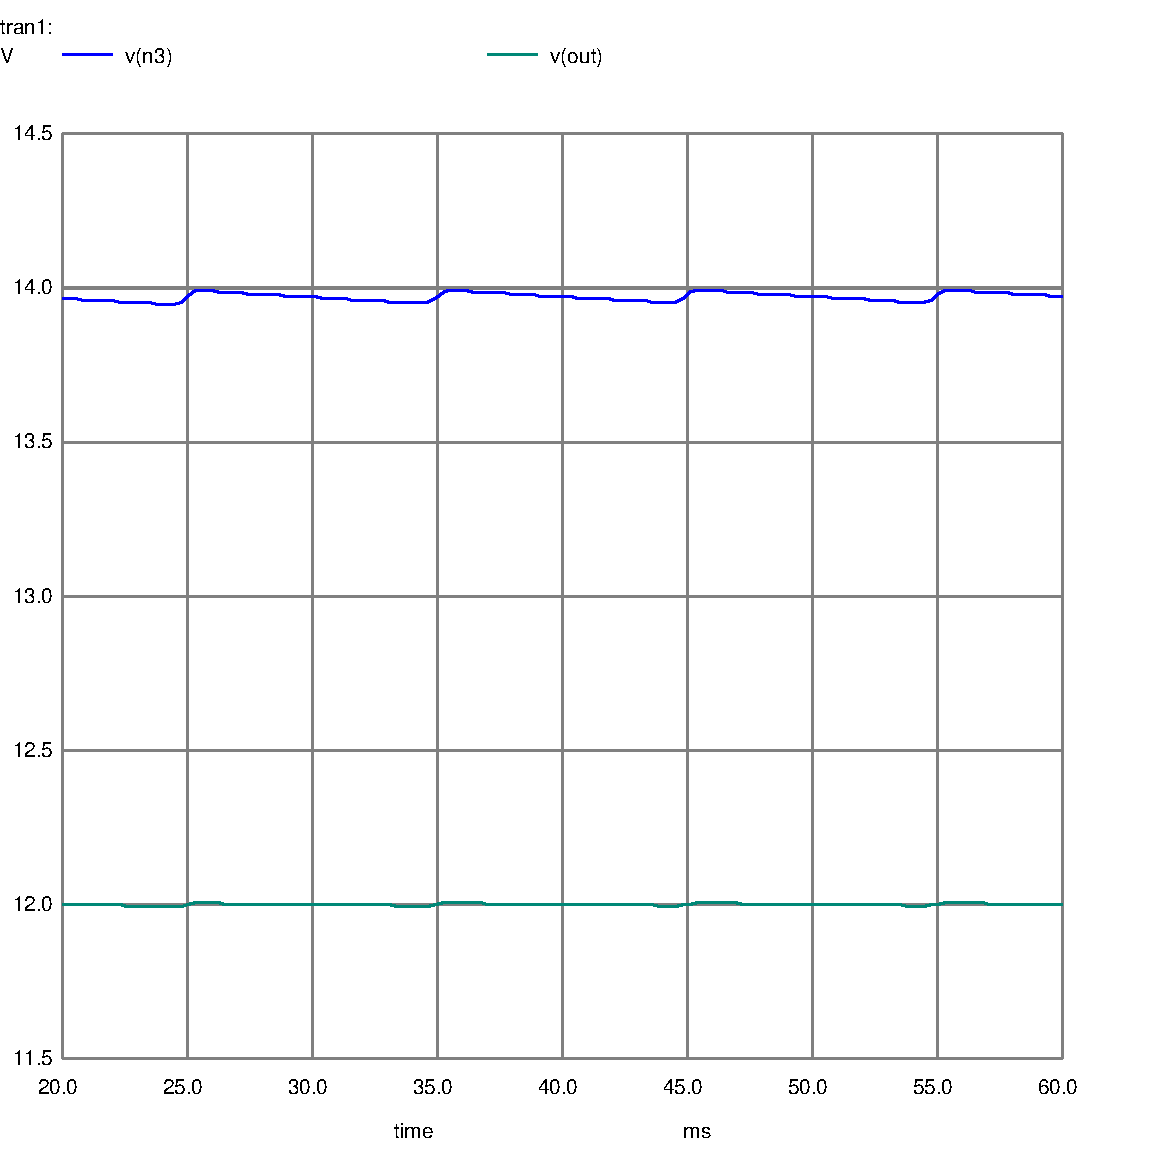
\includegraphics[scale=0.42]{Spice_t3_Zoom.pdf}
  \caption{Negative half.}
  \label{fig:33}
\end{figure}

\begin{figure}[h] \centering
  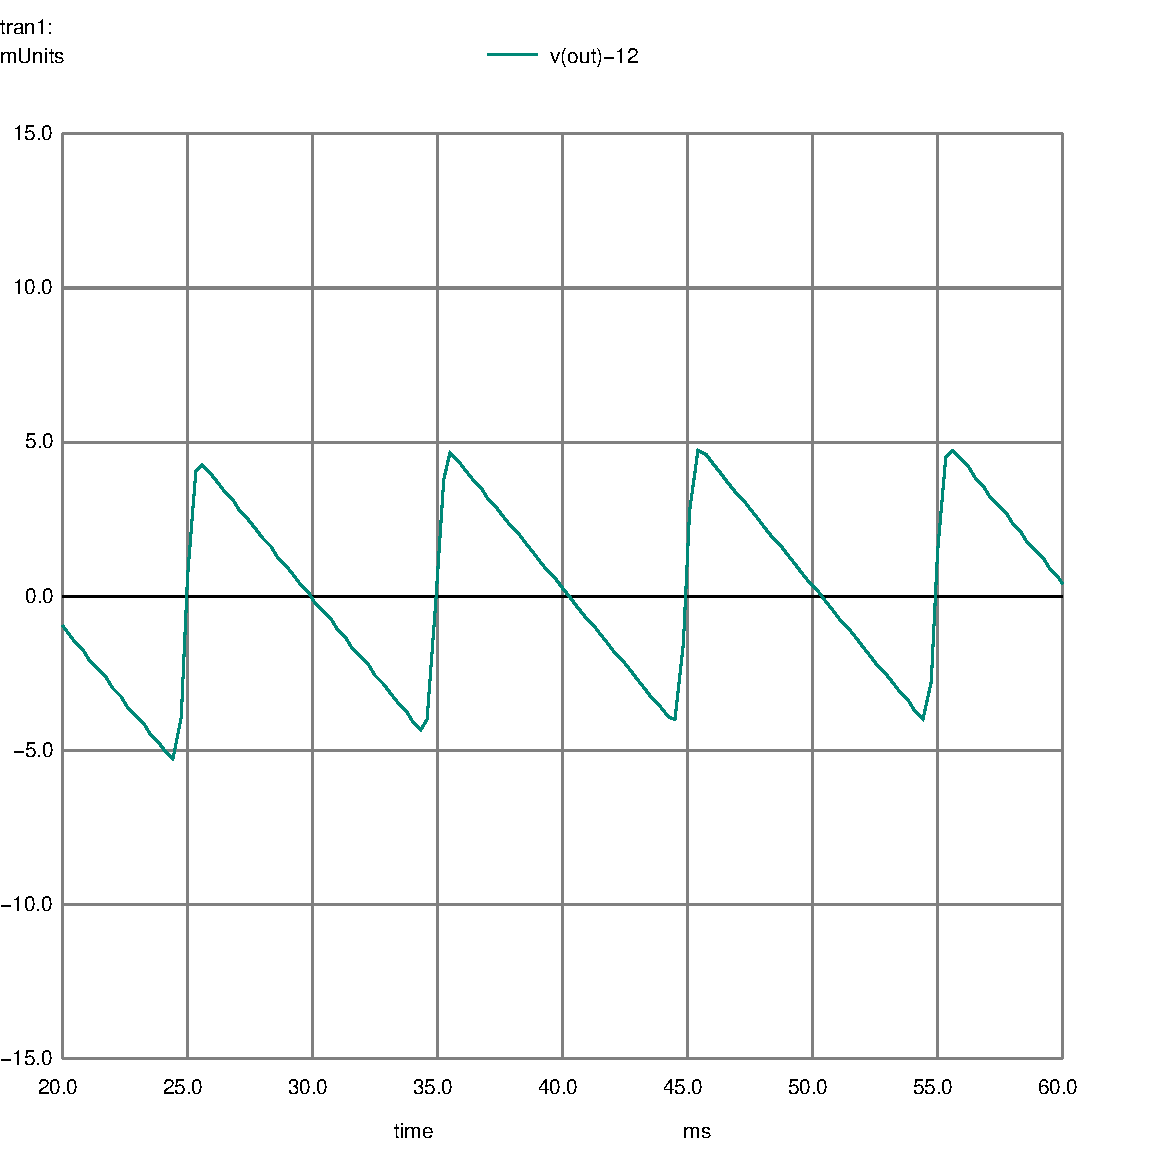
\includegraphics[scale=0.42]{Spice_t3_2_Zoom.pdf}
  \caption{Negative half.}
  \label{fig:44}
\end{figure}